\documentclass{beamer}

%Packages BEGIN
\usepackage{amsmath}

%Packages END

%Style setting BEGIN
\usetheme{Madrid} 
\usecolortheme{default} 
%Style setting END

\title{Anki Auto-lookup}
\subtitle{A convenient tool for English learning}
\author[Chiang, Wang, Hsu]
{Chia-Hsiang Chang\inst{1} \and Hao-Chien Wang\inst{2} \and Ding-Xiang Hsu \inst{2}}
 
\institute[NTU] % (optional)
{
	\inst{1}%
	Department of Electrical Engineering\\
	National Taiwan University
	\and
	\inst{2}%
	Department of Physics\\
	National Taiwan University
} 

\begin{document}

\frame{\titlepage} 

\begin{frame}
	\frametitle{Motivation}
	Anki: A cross-platform flashcard application, which supports images, HTML,
	\LaTeX, audio, etc.
	\begin{figure}[h]
		\centering
		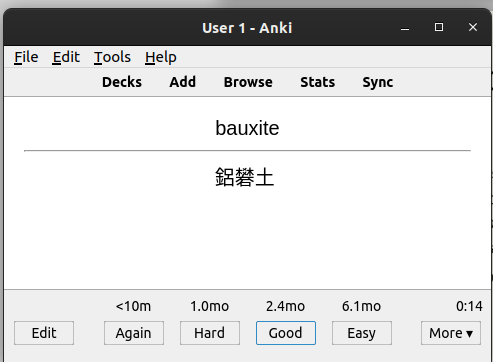
\includegraphics[width=0.55\linewidth]{./ankidesktop.png}
		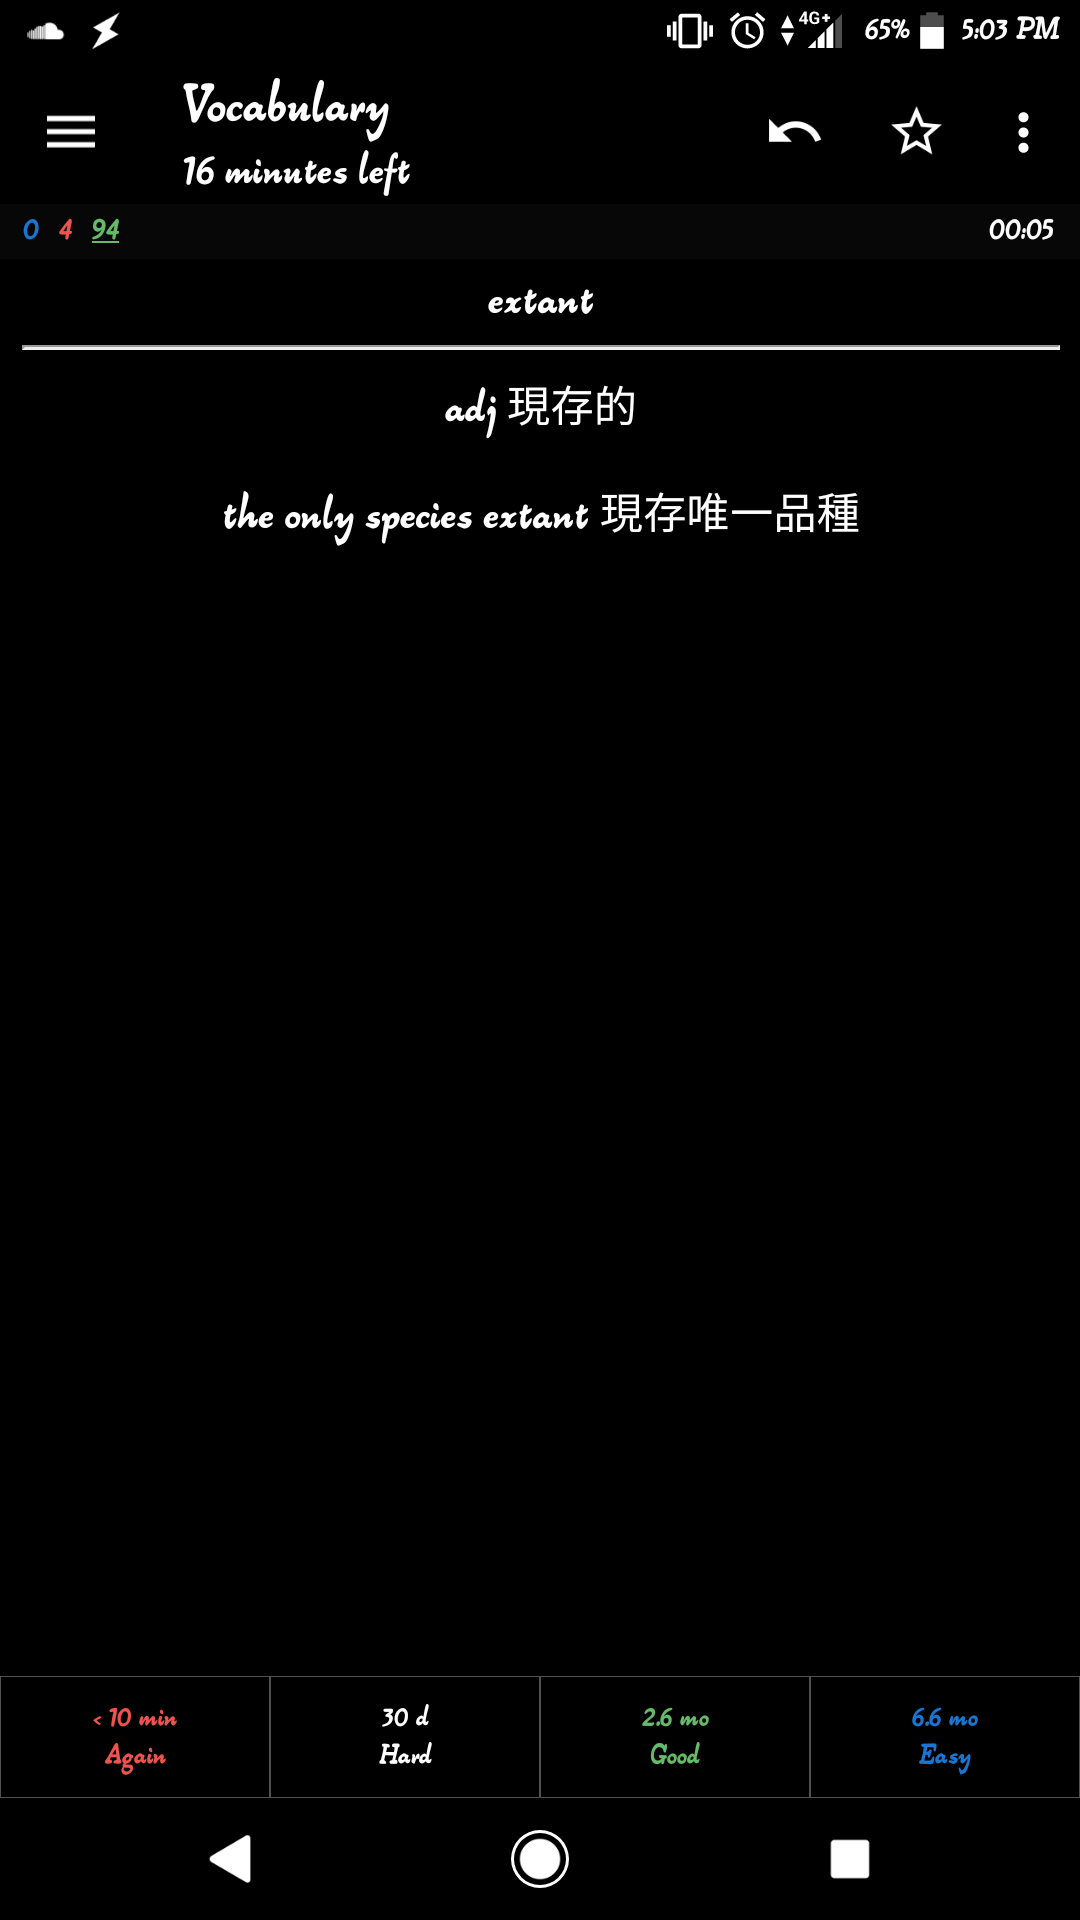
\includegraphics[width=0.28\linewidth]{./ankidroid.png}
		\caption{Anki on Ubuntu and Android.
		\label{fig:anki}}
	\end{figure}
\end{frame}


\end{document}
